\chapter{\uppercase{Literature Overview}}

\section{Stability of Dynamical Systems}

Stability of dynamical systems has a long history, appearing in the works of
researchers such as Routh \cite{Routh1877} and Hurwitz \cite{Hurwitz1895}.
%
Contemporary notions of stability in nonlinear systems generally rely on results
initially presented in the doctoral work of Aleksandr Lyapunov in his doctoral
thesis in 1892 \cite{Lyapunov1992}.
%
In said treatise, Lyapunov described two methods for analyzing the stability of
equilibrium points of ordinary differential equations.

The {\em first method}, sometimes called the {\em indirect method of Lyapunov},
provides a means for understanding the stability properties of an equilibrium
point by examining a linearization of the nonlinear system.
%
Due to the nature of linearization, the results of such an analysis only pertain
locally and within an unknown region about the equilibrium point.
%
Nonetheless, this method is well-known and sees widespread use due to its
simplicity and straightforward nature.
%

The {\em second method}, sometimes called the {\em direct method of Lyapunov}
involves the use of scalar-valued functions of the state of a system called {\em
  Lyapunov functions} which satisfy specific conditions that are set forth
later.
%
Through the use of these Lyapunov functions, it is possible to prove
stability not only locally but in a known region containing an equilibrium point
or even globally.
%
These functions are not unique and a major drawback to this method is the lack
of an algorithmic procedure for constructing valid Lyapunov functions.

Both methods are used in this work but for different purposes:
%
Lyapunov's indirect method is often used to analyze the stability of hybrid
systems by examining the stability of a linearization of the \Poincare{} map
about the equilibrium point; this will be explained in greater detail later in
this chapter.
%
Accordingly, the numerical simulations in this work will rely on this usage of
Lyapunov's indirect method.
%
In order to formally demonstrate the stability of energy shaping---the main
focus of this work---Lyapunov's direct method will be employed.
%
This method is often used in theoretical constructions and can also be used to
understand domain of attraction, although the particular usage will preclude
this type of application.

Lyapunov's work on the direct method established sufficient conditions for
stability but lacked the notion of {\em uniform stability} which was required
for establishing necessary conditions.
%
The results presented by Lyapunov lay essentially dormant for decades until
researchers began to investigate the ideas further.
%
From 1930's onward, researchers established additional results expanding on
Lyapunov's ideas.
%
Khalikoff \cite{Khalikoff1937} and Malkin \cite{Malkin1938} proved additional
theorems on stability which could be used to show stability in the sense of
Lyapunov with relaxed assumptions.
%
Masera \cite{Massera1949} provided more restrictive definitions, introducing the
notion of {\em equiasymptotic stability}.
%
Yet it wasn't until the assumptions of uniformity were formulated by Malkin
\cite{Malkin1954} that the necessary framework existed in which to formulate
converse theorems.
%
Barbashin and Krasovski\u{\i} further strengthed Malkin's result in \cite{Barbashin1954}.
%

After these observations were published, converse theorems followed shortly
thereafter thanks to researchers such as Kurzweil \cite{Kurzweil1956} and
Massera \cite{Massera1956}.
%
Converse theorems have seen substantial development and broad use since these results.
%
Hoppensteadt \cite{Hoppensteadt1966} presented constructions for singularly
perturbed systems in which he constructed a $C^{1}$ Lyapunov function, extending
existing work on singularly perturbed systems to unbounded time intervals.
%
Wilson \cite{Wilson1969} constructed a $C^{\infty}$ Lyapunov function for a
continuous vector field having an asymptotically stable invariant set.
%
Early results on converse Lyapunov functions for stability of sets are
summarized in numerous texts; see, e.g, \cite{Antosiewicz1958,Yoshizawa1975}.

In addition to providing necessary and sufficient conditions for stability,
researchers have also studied what conditions are necessary for solutions to be
integrable for all time.
%
Cesari provides conditions  for \cite[\S 1.5]{Cesari1971} for second-order
linear systems.
%
Strauss introduces $L^{p}$ stability to attempt to provide conditions for more
general systems in \cite{Strauss1965}.

As LaSalle points out \cite{LaSalle1964}, before the 1960's much of the work
done in the USSR was inaccessible to English-speaking audiences, but as the
decade progressed, this language barrier gradually dissipated.
%
An early text by LaSalle and Lefschetz (the first such text in English)
\cite{LaSalle1961} outlining the methods of Lyapunov stability theory contains
proofs which are accessible to those with less extensive mathematical
backgrounds.
%
Shortly thereafter, additional texts emerged including those of Krasovski\u{\i}
\cite{Krasovskii1963} and of Hahn \cite{Hahn1967}.

Additional information on the history of Lyapunov theory can be found throughout
the literature; see, e.g., \cite{Michel2007,Teel1999}.
%
Definitions of stability are ubiquitous in the literature; see, e.g.,
\cite{Khalil2002,Teschl2012,Vidyasagar1993}.

\section{Bipedal Robotic Locomotion}

%\textbf{JWG: In the following, I have started some of the editing. Hopefully I will have help!}

%\begin{itemize}

%\item Inverted Pendulum, hence no impacts. Include ZMP and Pratt's foot placement?

%\item Passive models, hence no control

%\item SLIP,

%\item Templates? Koditschek  <---------maybe goes into SLIP?

%\item Jogging Johnnie used  full feedback linearization for a fully actuated gait....not sure if impacts were addressed.

%\item What does this leave out? Russ Tedrake's linearization along a trajectory + LQR [which goes back to Song and Zefran in 2006.]

%\end{itemize}

%\begin{figure*}
%  \centering
%  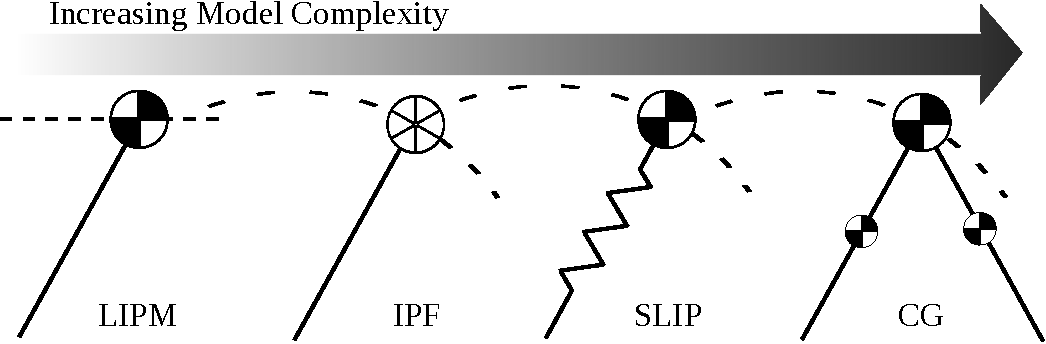
\includegraphics[width=1.0\textwidth]{biped-models}
%  \caption{Four low-dimensional models that are frequently used as approximate representations of walking robots. From left to right:
    %Linear Inverted Pendulum, Inverted Pendulum with Flywheel, Spring-Loaded Inverted Pendulum, Compass-Gait Biped
%    %
%    the Linear Inverted Pendulum Model (LIPM) lumps the mass of the robot at a point moving at a %constant height and assumes massless legs;
%    %
%    the Inverted Pendulum with Flywheel (IPF) relaxes the assumption on constant height and adds %a flywheel to account for internal angular momentum;
%    %
%    the Spring-Loaded Inverted Pendulum (SLIP) adds a spring to model a robot's legs as a %massless pogo stick;
%    %
%    and the Compass-Gait Biped (CG) treats a robot as a double pendulum with lumped masses on %the stance and swing legs.}
%  \label{fig:biped-models}
%\end{figure*}

%\section{Comments on the Literature}
%\label{sec:Literature}
Over the past fifty years, research into bipedal robots has come from a variety of perspectives: from passive walkers with simple mechanical designs to advanced multifunctional humanoids.
%
Myriad control designs have been introduced using models which vary from the simplified representations shown in \figref{fig:biped-models} to full-dimensional dynamic models as developed in \secref{sec:model}.
%
Proponents of simplified models point to the benefits of more tractable analysis, enhanced insight, and faster control law computation, whereas proponents of more complex models point to enhanced predictive ability and formal guarantees on stability.
%
In this section, some of the more common approaches to bipedal gait generation are examined with a particular emphasis on how the underlying modeling paradigms affect control design.
%
The book \cite{Westervelt2007} and the review paper \cite{Hurmuzlu2004} provide an extensive overview of the state of the art up to early 2006; further information is available in \cite{Full1999,Holmes2006,Wisse2007,Kuo2007,Siciliano2008,Chevallereau2009,Sadati2012} and the references therein.
% Remove papers which are not reviews. CHGRSHIH09

\subsection{Zero Moment Point and Linear Inverted Pendulum Models}

%\textbf{Ryan: I tried to make this coherent and have probably failed miserably. Please take a close look. Here are some remarks:}
%\begin{itemize}
%  %\item  Your original file is named LiteratureOverview\_v03\_originalByRyan.tex
%\item The original text did not relate ZMP to the previous section on modeling. I tried to fix that.
%\item Also, there are several ideas here...ZMP, LIPM, and humanoids. The first 2 are currently tied together. The general humanoid thing is just hanging.
%\item There was not statement about what exactly do we mean by ZMP control. I tried to fix that, but maybe I a%m not clear enough.
%\item The subsection is really on control methods. We probably should open with ZMP and relate that to LIPM, instead of the other way around.
%\end{itemize}

One of the most common control methods for bipedal locomotion is the ZMP control strategy.
%
Recall from \secref{sec:model:SS_FlatFeet} that the ZMP is the point on the ground at which the reaction forces acting between the ground and the foot produce no horizontal moment.
%
Traditionally, ZMP control strategies achieve walking by planning the motion of a robot's CoM such that the ZMP remains strictly within the convex hull of the stance foot in the case of single support (or convex hull of the stance feet, in the case of double support).
%
Under this condition on the ZMP, the stance foot remains flat on the ground and immobile (not rotating)---much like the base of a traditional manipulator robot---and hence the robot will not topple; see, e.g., \cite{Yamaguchi1999}.

In the special case of the Linear Inverted Pendulum Model (LIPM),
%
%When the height of the CoM is constant as in the LIPM,
%
the ZMP can be expressed explicitly in terms of the dynamics of the CoM via a linear ordinary differential equation (ODE).
%
There are key assumptions permitting this simplification, including representing a robot as a point mass with massless telescoping legs.
%
Additionally, the height of the CoM is assumed constant throughout a step.
%
Under these conditions, \cite{Kajita1991} showed that the robot model reduces to the LIPM.
%
%The ZMP control strategy uses the linear ODE to plan the motion of a robot's CoM such that the ZMP remains strictly within the convex hull of the stance foot in the case of single support (or convex hull of the stance feet, in the case of double support).
%
Because of their simplicity when combined, the ZMP control method and the LIPM have historically been tightly connected.
%
%One of the more popular models considered for bipedal walking is the Linear Inverted Pendulum Model (LIPM), which represents a robot as a point mass with massless telescoping legs.
%
%Importantly, this model assumes the height of the center of mass (CoM) and angular momentum about the stance foot are constant through a step.
%
%
While the model found its origins in the study of human posture and balance (e.g., \cite{Geursen1976,Winter1995,Patton1999}), it has also been the subject of much attention in bipedal walking; see, for example, \cite{Miura1984,Kajita2001,Kajita2010}.
%
%This simplified model is often used with control methods that generate walking gaits by controlling the ZMP.



Many of the early experimental results of bipedal robotic walking came from Japan, where Kato began working on the WABOT series of humanoid robots around 1970.
%
A full-scale anthropomorphic robot, WABOT-1, was reported in \cite{Kato1974} and it demonstrated primitive, statically stable walking while transporting objects with its hands.
% might be the first
%
Over a decade later, the ZMP technique was first demonstrated in practice on the WL10-RD biped in \cite{Takanishi1985}.
%
Interest in walking humanoid robots has continued to grow with researchers from around the world frequently developing newer generations like WABIAN-2, ASIMO, HRP-4, KHR-3, and Johnnie (\cite{Ogura2006,Sakagami2002,Kaneko2011,Park2005,Pfeiffer2002}).
%


In spite of the widespread success of ZMP methods, there are recognized limitations.
%
Gaits designed using this method generally do not take impacts into account, and thus the swing foot trajectory must be designed so that it will impact the ground with minimal velocity, which can be hard to achieve.
%
In addition, it is known that meeting the ZMP condition is not sufficient for asymptotic stability of a periodic walking motion (see \cite{Choi2005}).
%
Gait generation using ZMP has taken many forms:
%
\cite{Kurazume2003} used analytical solutions to the ZMP dynamics; \cite{Nagasaka1999} used the optimal gradient method;
%
\cite{Kajita1992} examined potential energy conserving orbits; \cite{Lim2002} computed ZMP-consistent trajectories offline and stabilized them using trunk motion;
%
and \cite{Nishiwaki2002} generated ZMP-consistent trajectories in real-time while walking.
%
Additional information on ZMP-based methods and related ground reference points is given in \cite{Goswami1999,Vukobratovic2004,Vukobratovic2006,Popovic2005}.

%Other contributions include \cite{Yamaguchi1999}.
%BHR-2 \cite{Jarfi2006}, SURALP \cite{Taskiran2010}.    china and turkey!!! also, REEM-B from Spain
%what about COMAN from Italy (no walking reported in publication?)?
%

\subsection{Nonlinear Inverted Pendulum Models}

In order to overcome limitations resulting from the simplicity of the LIPM model, researchers have considered more complex models.
%
\cite{Park1998} explored the Gravity Compensated LIPM which adds an additional point mass at the location of the swing foot to achieve higher modeling accuracy.
%
In \cite{Pratt2007}, the requirement of constant CoM height on the LIPM was relaxed leading to a nonlinear inverted pendulum model.
%
In another common model, a flywheel is added to the inverted pendulum;
%
examples can be found throughout the literature:
%
\cite{Stephens2011} used it for posture control,
%
\cite{Takenaka2009} used it to with on-line error compensation to mitigate the effect of modeling errors on gait generation,
%
and \cite{Komura2005} used it to simulate pathological gaits.
%
The various pendulum models have been widely used in analysis of push recovery and balance (\cite{Takanishi1990,Hof2005,Hyon2007,Stephens2007}).

%However, the capture point method is often used with simply the LIPM model (\cite{Englsberger2012}) to achieve walking.

%over the past decade, researchers have taken further forays into the feedback control of humanoid robots, examining aspects such as balance and push recovery \cite{PCDG2006,Stephens_humanoidpush2007,Pratt2012,Koolen2012}.
%
\cite{Pratt2006} considered a flywheel model in order to present the idea of the {\em capture point} -- a point on the ground on which a biped can step and come to a complete (upright) stop without falling over%
% -- building on the work of \cite{}
; additional information on capture points can be found in \cite{Koolen2012,Pratt2012}.
%
The capture point (\cite{Pratt2006a}) has gained recognition as a convenient method for stabilizing a biped.
%
%ntuitively, a capture point is a point on the ground where a biped can place its swing foot to be able to avoid falling over -- the set of all capture points is called the {\em capture region}.
%
This method, which considers a robot as an inverted pendulum with a flywheel, has been used not only for standing but for robust walking as well.
%
Because the model makes many simplifying assumptions, the capture regions -- the set of all capture points -- can have a large error and this has motivated the combining of capture point with learning in, e.g., \cite{Rebula2007}.

\subsection{Raibert Hoppers and SLIP Models}

Raibert observed that hopping and running can be represented by a low-dimensional model with springs and built a pneumatically actuated planar monopod with a pogo-stick (springy) leg that was able to run%
%
\footnote{Roughly speaking, running consists of a stance phase with one foot on the ground followed by a flight phase with no feet on the ground; hence hopping on one leg and running on two legs are closely related.}\xspace
%
at a speed of 1 m/s (\cite{Raibert1984,Raibert1984a,Raibert1986}).
%
This was followed by a 3D hopper that was able to run without being constrained to the sagittal plane (\cite[Chap.~3]{Raibert1986}, \cite{raibert:dbu}) as well as multi-legged robots \cite{raibert1986a,Raibert1990,Hodgins1991}.
%

This body of work gave rise to the Spring-Loaded Inverted Pendulum (SLIP) model,
which has been shown to approximate the body center-of-mass (CoM) motion during
\textit{steady-state running gaits} of a wide diversity of terrestrial animals
\cite{Blickhan1989,Mcmahon1990,Farley1993,Full2000,Dickinson2000,Seyfarth2002}.
%
Successful running robots, such as the Planar Hopper, ARL Mono pod II and CMU Bowleg Hopper, also exhibit SLIP model behavior (\cite{Raibert1986,Zeglin1998,Ahmadi2006}).
%

The control of these robots has been based on Raibert's original control ideas,
which can be decomposed into three subtasks dedicated to (a) forward propulsion
of the robot at the desired speed, (b) regulation of the vertical hopping height
of the body, and (c) keeping the body at a desired posture (\cite{Raibert1984},
\cite[Ch. 2]{Raibert1986}).
%
To control the forward speed, the controller places the toe at a desired position with respect to the center of mass during flight.
%
To regulate the hopping height, the length of the leg at the bottom of the stance phase is adjusted by giving a fixed amount of thrust.
%
Finally, to control the pitch attitude of the body, the controller employs hip torque during stance.
%
The inclusion of springs into legged robots with revolute knees seems to have started with spring flamingo and spring turkey as described in \cite{HOHUBA92,PRPR99,PR00,PRCHTODIPR01}.
%
These robots used a type of series elastic actuator (SEA) designed for force control as opposed to energy storage. %is it necessary to say this? JWG re-worded. helps to tie in with MABEL.
%
The recent COMAN robot discussed in \cite{robots_coman} includes passive compliance to reduce energy consumption during walking.


\subsection{Passive Walkers and the Compass-Gait Biped}

%\textbf{JWG: key points are: no actuation, but uses full hybrid model. Compass-gait biped is an inverted pendulum }

At the other end of the spectrum, instead approximating complex bipeds with simplified models, some researchers have opted to design robots with dynamics that approximately realize a simplified model.
%
For these bipeds, dynamic stability is achieved as much as possible through mechanical design instead of feedback control.
%
Though comparatively less complex in terms of the models studied, many of the formal methods developed on simple bipeds still enjoy use in complex systems.
%
However, the simpler design facilitates more complete modeling and, indeed, control researchers who follow this path often consider impact dynamics, thereby taking into account the full hybrid model which is generally omitted from analysis of controllers designed using the LIPM.
%

\cite{Mochon198049} concluded that the swing phase of human walking is similar to a double pendulum, pointing to the passive nature of human walking and the importance of mechanism design.
%
In the late 80's, McGeer analyzed and built planar, passive bipedal walkers, i.e., {\em no actuation}, which could walk stably down shallow slopes, starting with the compass gait walker (which is simply an inverted pendulum) in \cite{MC90} and later adding knees in \cite{mcgeer:kneed}.
%
This gave rise to the terminology {\em passive dynamic walking}.
%
Subsequently, robots with this general principle at their core have been constructed, as described in \cite{CORUTEWI05}, based on injecting small amounts of energy into passive-type bipeds.
%
The result is very ``human-looking'' walking, but the remarkable elegance and economy of these walkers comes at the cost of poor ability in achieving tasks other than walking at a fixed speed; they cannot climb stairs, pause, turn or run.
%

Additional work was later done to analyze the properties of passive dynamics walkers, for instance, in \cite{ESGO94,GACHRUCO98,BORZOVAE04}.
%
In terms of control, \cite{SP99} looked at passive dynamic walking with energy-based methods to design passivity-based control strategies such as controlled symmetries, introduced in \cite{SPBU05}.
%, which was later used to obtain anthropomorphic foot action in \cite{SA:CDC09-1,SA:CDC09-2} and recently extended to underactuated bipeds in \cite{Hu20111605}.
% maybe this doesn't go here, but maybe good to put newer stuff
%
%
%Other methods
%
%A thorough analysis of the compass-gait biped and its stability properties was later provided by Espiau and Goswami \cite{ESGO94}.
% don't really need the above sentence
Other important contributions to passive dynamic walking are given in \cite{KUO99,KUO02,ANDERSONS05,WIVDL07}.
%

%\subsection{Foot Placement}
\subsection{Quadratic Programs and Lyapunov Funnels}

%\textbf{JWG: disucss how early implementations used offline trajectory computation, while more recently, on-line planning via an linear inverted pendulum model and a QP are used (Weiber)?}

Early implementations of ZMP-based controllers used offline trajectory optimization to generate center of mass trajectories on the basis of the LIPM and generally ignored impact dynamics in the control design. Modern methods have achieved improved control by formulating the control problem as a {\em quadratic program} (QP), allowing gait replanning on the fly and improving stability properties (\cite{KuKoIk02,stephens2010push,herdt2010online}).
%

Similarly, sums of squares methods, also formulate trajectory generation as a convex optimization (\cite{TeMaToRo2010}).
%
One elegant method which provides formal guarantees on stability is outlined in \cite{MaAhTe2013}.
%
The procedure investigates the notion of controllability, composing sequential funnels (verified with sum of squares Lyapunov inequalities), which each lead to a predefined goal set.
%
This allows one to create a trajectory with guaranteed stability properties: at any given point in time, the system is within one of the known funnels (regions of attraction).
%
By using the sum of squares formulation, the trajectory optimization becomes more tractable, making verification of stability feasible for low-dimensional models.






%------------------------------------------

%McGeer was studying passive walking and reported that a compass-gait biped can walk down shallow slopes with no actuation \cite{MCG88,MC90}. A thorough analysis of the compass-gait biped and its stability properties was later provided by Espiau and Goswami \cite{ESGO94}. This idea of passive dynamic walking was later used to \cite{BORZOVAE04}

% \cite{KAMO84}
%There is a noticeable dichotomy in the field of robotics with some researchers pursuing advanced mechanical designs with humanoid characteristics and others favoring minimalist designs conducive to natural and efficient locomotion.

% Ben's paper, Matt's, TAC CLF in Section 6.4
